Basic scheme\footnote{
S. Tang; J.M. Liu,
 Chaotic Pulsing and Quasi-Periodic Route to Chaos in a Semiconductor Laser with Delayed Opto-Electronic Feedback    
}:


\phantom{42}

\begin{minipage}{0.4\textwidth}
\begin{figure}[h]
    \centering
    \hspace{-10 mm}
    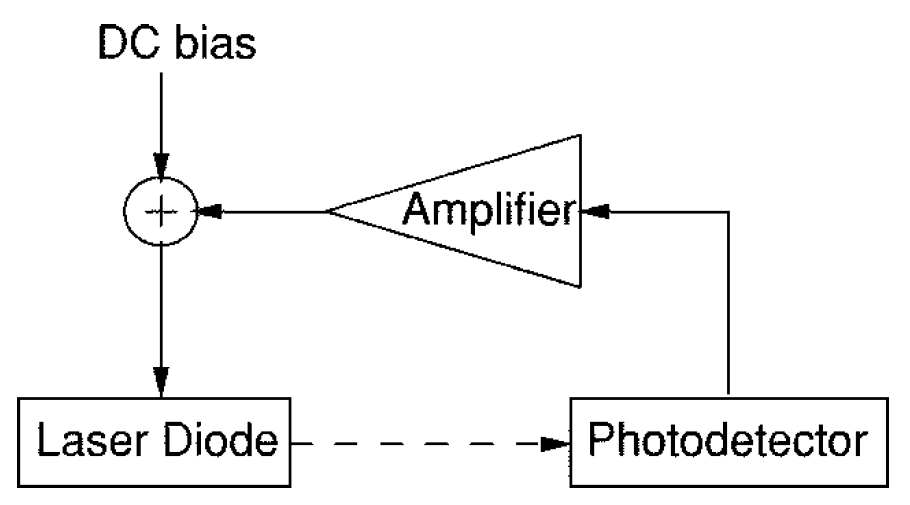
\includegraphics[width=1.2\textwidth]{images/SS.png}
    \caption{Schematic experimental setup}
\end{figure}
\end{minipage}
\hfill
\begin{minipage}{0.55\textwidth}

\textbf{Laser} -- single-mode DFB laser diode (1300 nm);

\textbf{Light output detector} -- high-speed InGaAs photodetector;

\end{minipage}


\textbf{Important}: it is suitable for any other semiconductor laser with an active medium.



